% Target: 20ish pages total; 13 pages of text, 7 pages of images
\chapter{Load Balancers and Their Placement}
In this chapter we describe our chosen approach for improving the performance of network bound workloads in serverless edge computing environments. We start by explaining our considerations when developing our approach in the context of a serverless edge computing system, and showing in what way our solution changes the system. From there, we go into detail about how the load balancing mechanism of our solution works, how it is different from currently employed methods, and how the choices made in regard to the load balancing method inform other parts of the proposed approach.
Lastly, we go into our approach to scaling and scheduling load balancers among the nodes present in the serverless edge computing system. We make use of osmotic scaling and scheduling, a method previously outlined in existing literature. Using this idea of osmotic scaling and scheduling, we provide a concrete implementation of such an approach for placing and deciding on the number of load balancers in the system. The implementation is designed with current state of the art systems such as Kubernetes as its basis, and can thus be used as a reference implementation for use outside of a simulation context. The approach also addresses the challenges of edge computing environments that make current methods, developed with the cloud in mind, unsuitable. Specifically, our approach addresses issues of location awareness, device and network heterogeneity, and dynamically changing workload conditions.
% Target: 2ish pages \w graphics
\section{Concept}
% Note: mention that in our context load balancing and entry-gateway are sort of equivalent. Show their relation a bit
% Note: Mention that our approach uses the method of using real-life experiments to inform simulation

To understand the approach we first take a step back to view the boarder technical context the solution addresses and is built around.
As previously outlined, our solution aims to improve the performance of network bound workloads.
In the context of serverless edge computing systems network bound workloads are characterized by the network being the main or a significant contributing factor to the overall response time.
\begin{figure}
    \centering
    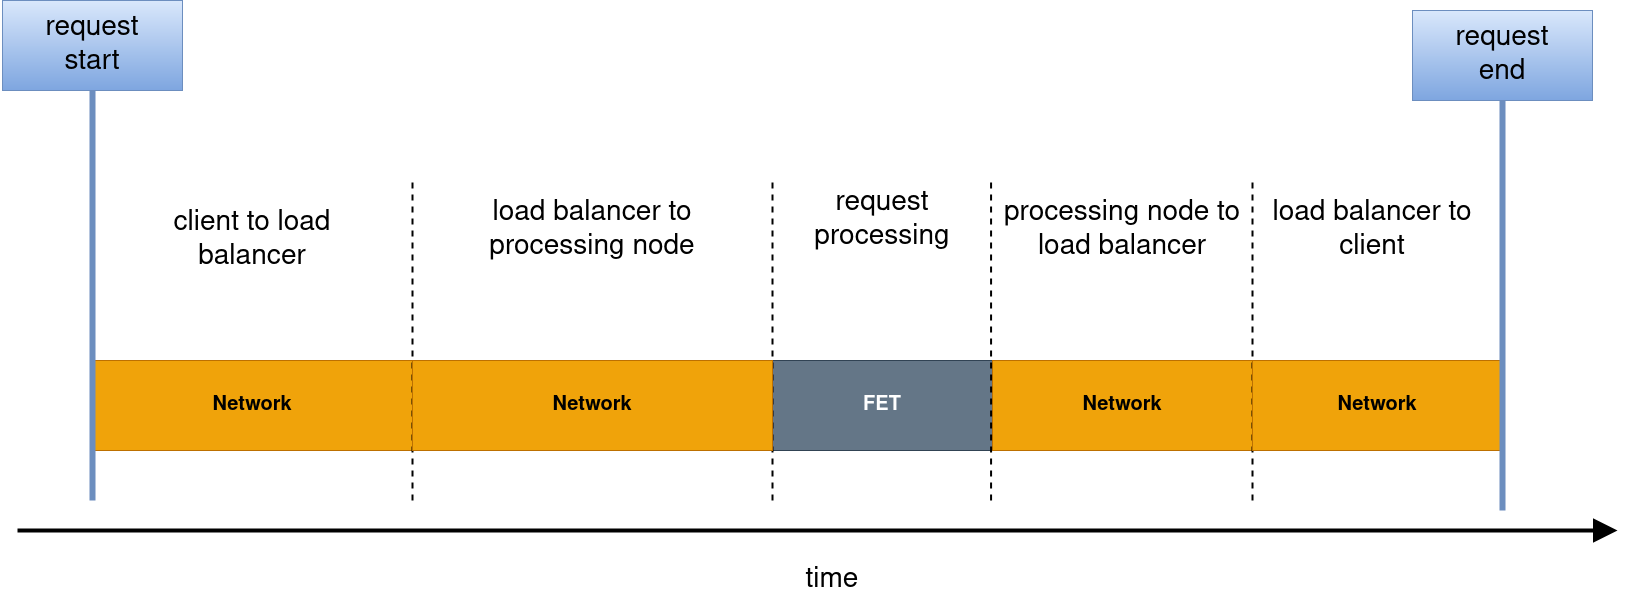
\includegraphics[width=14cm]{graphics/diagrams/request_overview.png}
    \caption{A generic view of the different parts that make up the total request processing time from the perspective of our approach}
    \label{fig:request_net_fet_overview}
\end{figure}
In Figure \ref{fig:request_net_fet_overview} we can see the different processing steps we consider for a request.
A network bound workload in this sense is one where the time taken up by the network portion of handling the request is proportionally speaking significantly larger than the portion taken by the \gls{fet}.
This is typically the case because either the request contains a lot of data that needs to be transported, or because the \gls{fet} is very short.

The primary way by which our approach improves the response times of network bound workloads is thus by reducing the amount of time spent on the network transfer portion of handling a client request.
While optimizing \glspl{fet} is not the primary objective of our approach, at least from a systems design perspective, it still has the potential to additionally reduce \glspl{fet} compared to current methods.
We consider the structure and makeup of the serverless computing system to be a given factor. As a result our approach aims to reduce network times not by changing the network makeup itself, but by utilizing the existing resources as effectively as possible. From a network-optimization perspective this means that each request should take an optimal path from  the client to the node where the request is ultimately processed. 

\begin{figure}
    \centering
    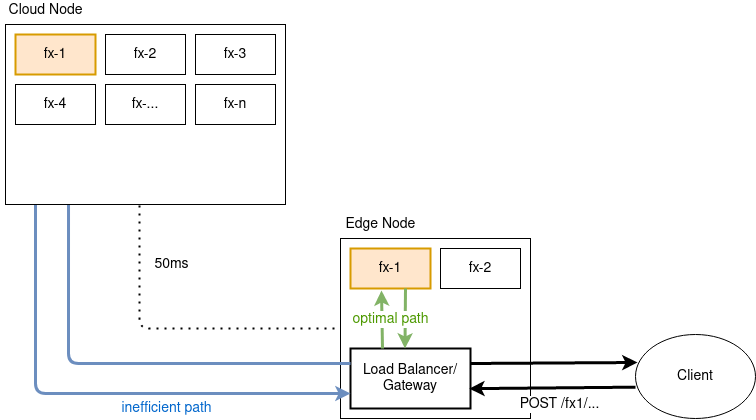
\includegraphics[width=12cm]{graphics/diagrams/efficient_path_example.png}
    \caption{Example diagram showing efficient and inefficient request routing based on network delay. "fx-1" through "fx-2" denote different types of function, and the dotted line denotes a network link between the cloud and edge node with a latency of 50ms}
    \label{fig:efficient_path}
\end{figure}

As can be understood quite intuitively in Figure \ref{fig:efficient_path}, round robin load balancing will in many cases lead to clearly suboptimal choices in terms of incurred network delay. The figure also shows the three key components we consider when trying to make network location based decisions: The client, the load balancer, and the node. Because our approach solely considers application level load balancers, since serverless platforms typically require these for their advanced routing decisions, any given request takes a path from the client to the load balancer, then to the selected upstream node, and back the same way.

Subsequently we want to incur the minimal amount of delay possible from both the hop between the client and load balancer, as well as between the load balancer and upstream node. Our proposed approach handles these two kinds of hops separately, at least for the most part. Since the scope of this work does not include optimizing the location of the serverless function instances themselves, this means we can improve performance through the following methods:
\begin{enumerate}
    \item \textbf{Intelligent load balancing decisions:} load balancers should choose upstream nodes that are both close in the network, and have \glspl{fet} short enough as not to negate the performance won through network proximity
    \item \textbf{Effective placement of load balancers:} the scheduler of the serverless system should place load balancers at locations in the network where they are in close proximity to clients and serverless function instances requested by these clients
    \item \textbf{Efficient scaling of load balancers:} the amount of load balancers should be high enough to provide the needed performance improvement, but not so high that the resources consumed by the load balancers diminish or even negate that effect
\end{enumerate}
In our approach the first method is provided by the load balancer itself. It is continuously updated with information where function instances, typically also referred to as \textit{replicas}, are located. Based on this and other information gathered by the load balancer, it tries to make decisions that lead to faster overall request responsiveness by selecting upstreams that are close and provide fast \glspl{fet}.

The other two methods are handled by the osmotic joint scaling and scheduling component of our approach. While the different methods of improvement are split between these two components of our proposed solution, this does not mean that they are completely separate from each other. Naturally the scheduling and scaling decisions will influence the way in which the placed load balancers work, while these in-turn affect the data gathered for and available to the scaling and scheduling component. The specifics of these two components will be discussed in the next two sections. 

It is also important to note that a significant amount of the approaches' implementation details are not chosen arbitrarily, but are rather the result of continuous cycle of experimentation and evaluation. While not detailed in the approach, the evaluation, result, and discussion chapters of this thesis include some of these experiments, in particular those that give additional insight into the problem domain and yielded results useful beyond informing this specific approach.
% Target: 8 pages with figures
\section{Load Balancers}
In this section we describe the role the load balancer plays in the context of our approach, how it is related to the underlying serverless platform, and the details of how it is implemented.

\subsection{ Definition \& Role In a Typical Serverless Framework}
First, we want to discuss what component exactly we mean by \textit{load balancer}, and how it functions in the context of a serverless framework. While our approach is not tied to any specific serverless framework, implementation, or technology, we developed it with their general concepts and functioning in mind. Because of this we feel that is helpful and informative to explain the components of our system in the context of an actual implementation, since this helps understand the abstract role these components play. In addition this is helpful for anyone who might want to integrate our approach into a production ready serverless edge computing platform.

As previously mentioned there are a number of different serverless frameworks, some free, some open source, some commercial, and some that fall in-between \cite{aws-lambda}\cite{azure-functions}\cite{openfaas-gateway}\cite{kubeless}\cite{openwhisk}.
We choose OpenFaaS\cite{openfaas}
as our reference implementation of a serverless framework because it is open source, allowing us detailed understanding of its inner workings, because it has been extended, for edge computing, and because it builds on and makes use of well established technologies in the same way other serverless frameworks do\cite{kubeless}\cite{openwhisk}, thus making it representative for the space.


\begin{figure}
    \centering
    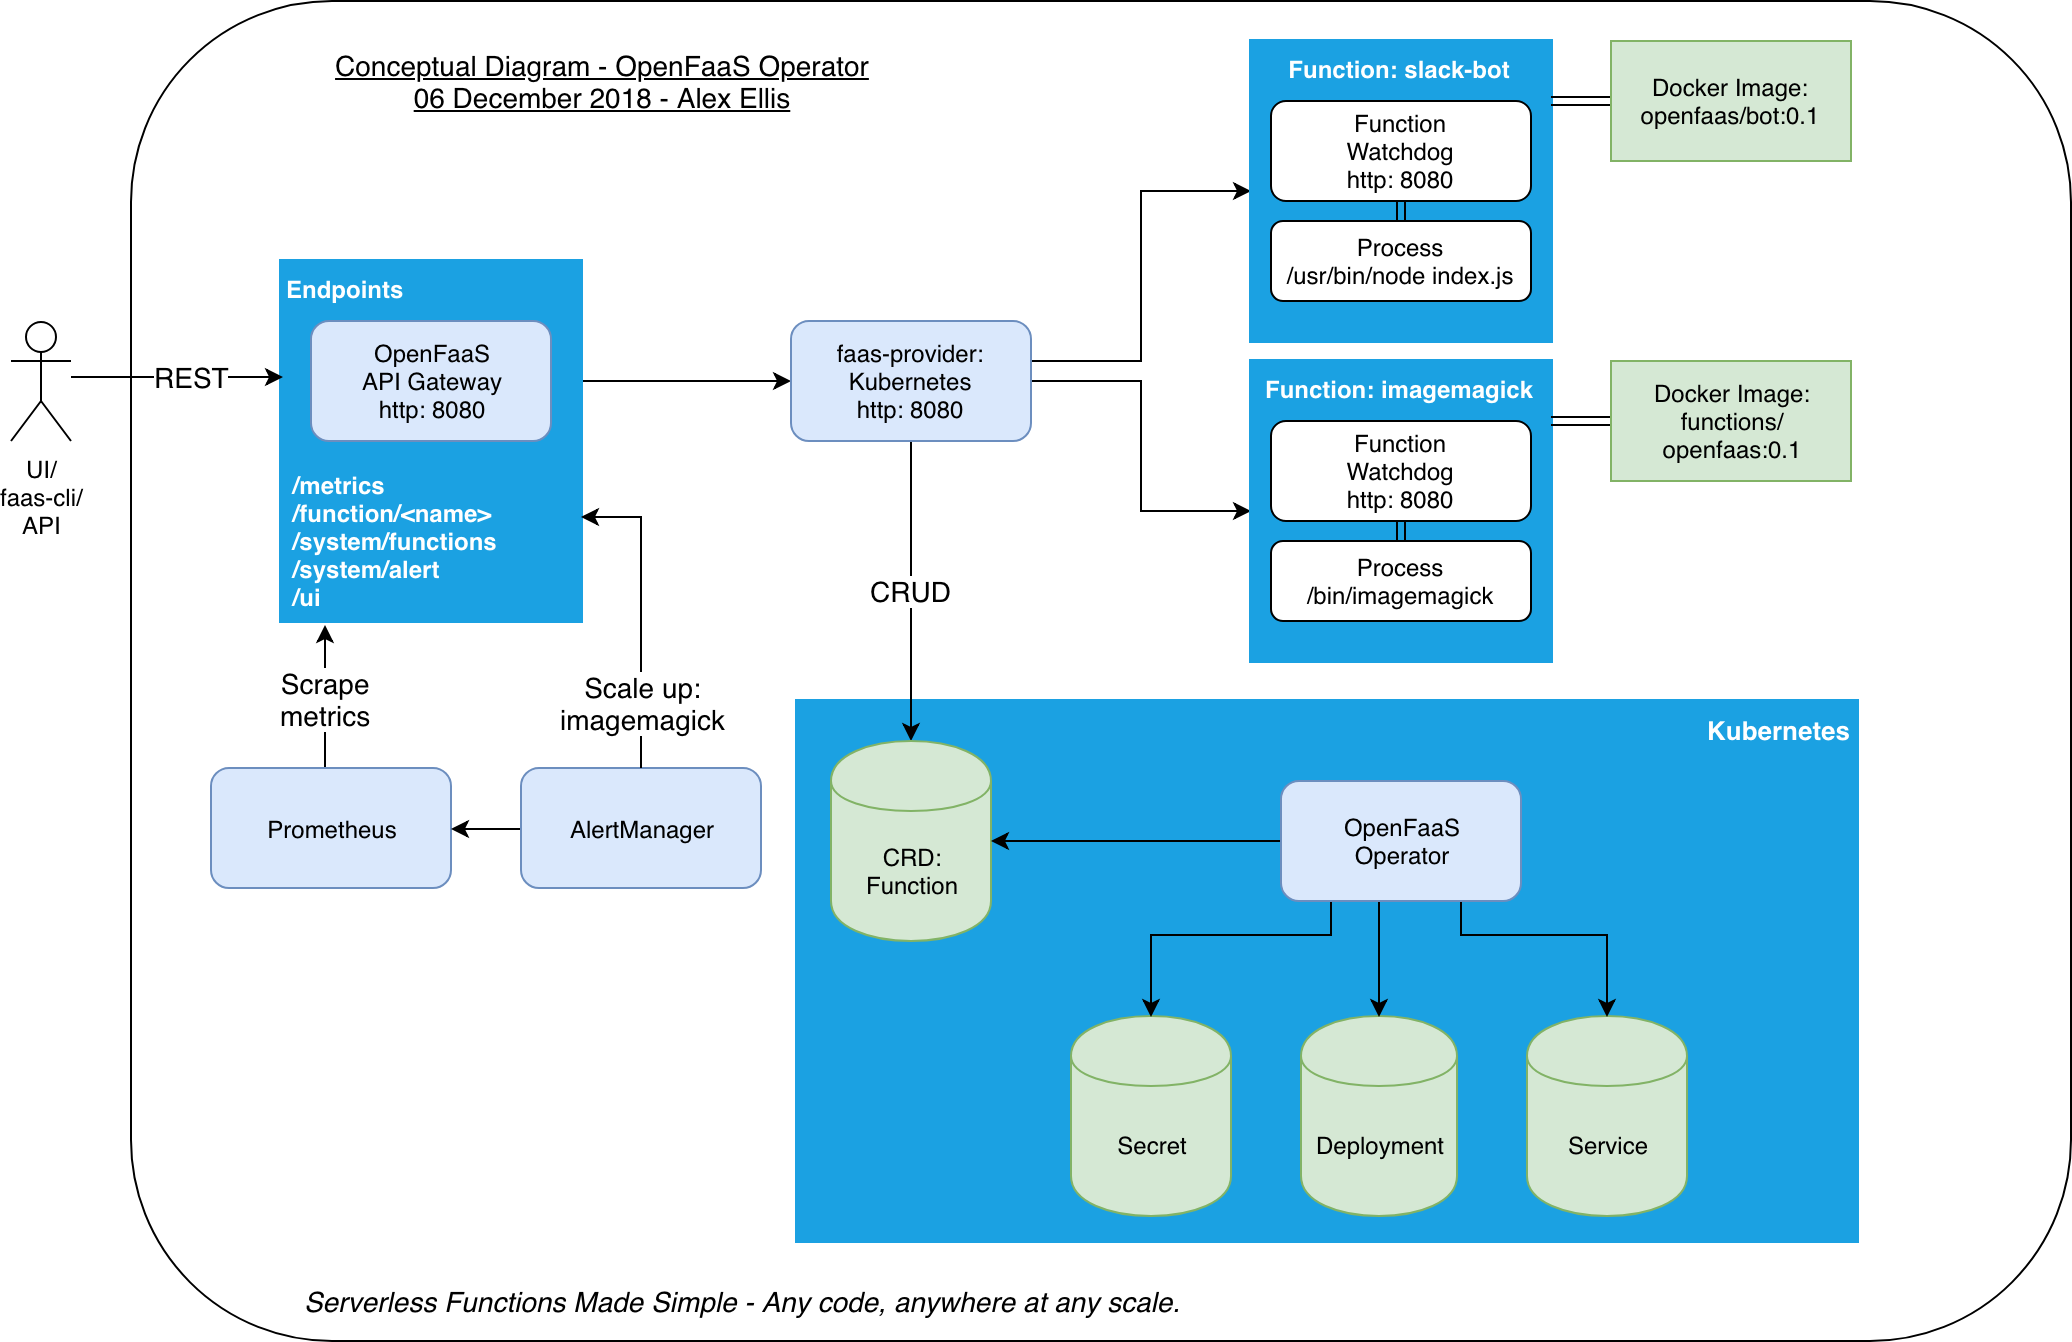
\includegraphics[width=14cm]{graphics/diagrams/openfaas-gateway-architecture.png}
    \caption{Diagram showing the architecture and components of OpenFaaS, in particular the OpenFaaS API Gateway. Taken from the official OpenFaaS architecture documentation\cite{openfaas-gateway}}
    \label{fig:openfaas-gateway-diagram}
\end{figure}


As mentioned in the background chapter, OpenFaaS uses Linux containers to run functions, and in turn Kubernetes to manage these containers. To clarify the role our load balancer would take in a serverless system, we describe how it would affect OpenFaaS. By default OpenFaaS employs a component they call \textit{API Gateway}. This API Gateway is the component which first receives \textbf{all} client requests, and then continues to send them on to the corresponding functions, while at the same time collecting metrics used by the system for tasks like auto-scaling. Figure \ref{fig:openfaas-gateway-diagram}, which is taken directly from the official OpenFaaS documentation shows the interactions with the other components of the system. Since the API Gateway is just another container running in Kubernetes\cite{kubernetes}, and failover capability is a concern, there can be multiple instances of the API Gateway running at any given time.
As discussed a major reason for the sub-optimal performance of network bound workloads in edge scenarios is the lack of efficient request routing.
In the case of OpenFaaS this stems from it delegating networking and routing tasks to Kubernetes, since it is the underlying container orchestration platform. This applies to both the initial ingress into the cluster, as well as to how the API Gateway forwards client requests to the relevant replicas to be processed. Kube-proxy, the component of Kubernetes which handles networking and routing tasks, will default to the round-robin policy of selecting upstreams. While it is possible to set up kube-proxy in a way that will prefer nodes in the same zone based on a label, this functionality is built around cloud based deployments and is insufficient to address the heterogeneity in networking and compute power introduced by edge computing. This defaulting to round-robin means that in effect, serverless frameworks such as OpenFaaS route the requests basically at random between the entry point in the network and the API Gateway, and then from the API Gateway to the relevant function.\\
In our approach the load balancer takes the role the API Gateway has in OpenFaaS. It is characterized by being
\begin{enumerate}
    \item the entry point for the client to the serverless system, meaning there are no network hops between the load balancer instance and the node the request originally arrived at, and
    \item directly forwarding requests to the corresponding serverless function instances.
\end{enumerate}
When implementing our proposed approach in practise this would mean that the serverless framework would have to be adapted to fulfill these conditions for the load balancer. If these conditions aren't met, this would likely negate the positive affect our approach has on performance.

As an example in the case of OpenFaaS, referencing the OpenFaaS architecture in Figure \ref{fig:openfaas-gateway-diagram}, this could be realized in the following ways:
\begin{enumerate}
    \item API Gateways and load balancers are scaled and scheduled together, meaning they are always co-located on the same node. The API-Gateway would then still first receive requests and handle implementation specific tasks for the serverless system, but then forward the request to the load balancer instance on the same node, which then decides on further request routing.
    \item The load balancer is the new entry point for clients, effectively replacing the API Gateway. In this scenario the load balancer and API Gateway would also be altered such that metrics and information relevant to the system could be collected by the load balancers and forwarded to API Gateway instances, which then handle them as before.
\end{enumerate}

\subsection{Load Balancing Concepts}

% Target: 8 pages with figures
\section{Scaling and Scheduling}
